\chapter{Edge Detection}

\section{What is an Edge?}

“边缘”是图像中的一个区域,在这个区域中,沿着图像的一个方向,
像素强度值 (或者说对比度) 发生了“显著”的变化,而在其正交方向上,
像素强度值 (或对比度) 几乎没有变化.

\section{Criteria for Optimal Edge Detection}

\begin{equation}
\text{Accuracy}=\frac{\text{TP}+\text{TN}}{\text{TP}+\text{FP}+\text{TN}+\text{FN}} 
\end{equation}

\begin{equation}
\text{Precision}=\frac{\text{TP}}{\text{TP}+\text{FP}} 
\end{equation}

\begin{equation}
\text{Recall}=\frac{\text{TP}}{\text{TP}+\text{FN}}
\end{equation}

Precision 和 Recall 都代表着你检测出的真正边缘所占比例,但是 Precision 的分母
是你检测出的边缘,Recall 的分母是真正的边缘.

\section{Non-Maximal Suppression (NMS)}

非最大值抑制,顾名思义,就是抑制非最大值,这里的最大值指的是梯度的局部最大值.

在计算出了所有点的梯度之后,会有很多像素的梯度大于设定的阈值,而我们希望最后得出的边缘像素真的看起来
像一条线而不是一块区域,所以 NMS 的目的是为了抑制那些不是边缘的像素,只保留那些是边缘的像素.

\begin{figure}[htbp]
    \centering
	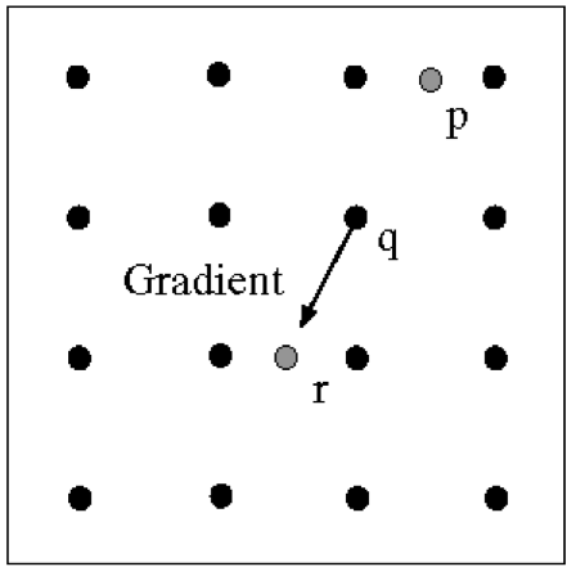
\includegraphics[scale=0.2]{figures/NMS.png}
	\caption{NMS示意图}
\end{figure}

对于一个边缘像素的候选点,我们认为它是边缘当:它比它梯度方向的两个点 $q+\nabla q$ 和 $q-\nabla q$ 的梯度值大,
也就是这个点的梯度大小是局部最大值的时候.

\begin{figure}[htbp]
    \centering
	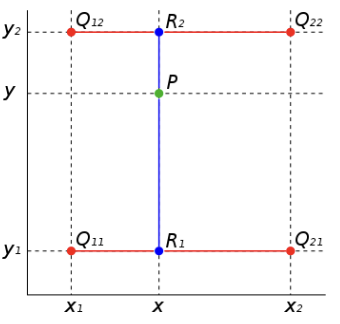
\includegraphics[scale=0.4]{figures/bilinear.png}
	\caption{双线性插值}
\end{figure}

计算这个点梯度方向的点的梯度值可以使用双线性插值法,就是把这个点周围的四个点的梯度按照横纵距离反比加权.

当然,NMS 是一个思想而不是针对边缘检测的算法,比如对于 keypoint detection,object detection (like YOLO) 都可以使用 NMS,
实现的思路都很类似,使用一个打分函数看这个备选点 (bounding box) 是不是比跟它相邻 (冲突) 的点 (bounding box) 好,如果是就保留,否则就抑制.

\section{A Simplified Version of NMS}

\begin{figure}[htbp]
    \centering
	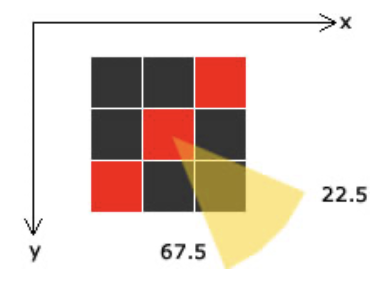
\includegraphics[scale=0.55]{figures/simple_NMS.png}
	\caption{简化版本的双线性插值}
\end{figure}

一个 NMS 的简化版本是把双线性插值省去,直接让这个像素的梯度大于它梯度方向的那两个相邻像素的梯度.

\section{Hysteresis Thresholding}

使用高阈值 (maxVal) 开始边缘曲线,使用低阈值 (minVal) 继续它们.

\begin{itemize}
    \item Pixels with gradient magnitudes > maxVal should be reserved.
    \item Pixels with gradient magnitudes < minVal should be removed.
\end{itemize}

How to decide maxVal and minVal? Examples:

\begin{itemize}
    \item maxVal = 0.3 $\times$ average magnitude of the pixels that pass NMS
    \item minVal = 0.1 $\times$ average magnitude of the pixels that pass NMS
\end{itemize}
